\section{結果}
\subsection{thorとoptparseのコードの比較}
\subsubsection{Thorとは}
Thorとは,コマンドラインツールの作成を支援するライブラリのことである. gitやbundlerのようにサブコマンドを含むコマンドラインツールを簡単に作成することができる.

\paragraph{Thorの基本的な流れ}
\begin{enumerate}
\item Thorを継承したクラスのパブリックメソッドがコマンドになる
\item クラス.start(ARGV)でコマンドラインの処理をスタートする
\end{enumerate}
\subsubsection{optparseとは}
optparseモジュールとは,getoptよりも簡便で,柔軟性に富み,かつ強力なコマンドライン解析ライブラリである.
optparseでは,より宣言的なスタイルのコマンドライン解析手法,すなわちOptionParserのインスタンスでコマンドラインを解析するという手法をとっている.
これを使うと,GNU/POSIX構文でオプションを指定できるだけでなく,使用法やヘルプメッセージの生成も行える.

\paragraph{optparseの基本的な流れ}
\begin{enumerate}
\item OptionParserオブジェクトoptを生成する
\item オプションを取り扱うブロックをoptに登録する
\item opt.parse(ARGV)でコマンドラインを実際にparseする
\end{enumerate}
\subsubsection{コードの解説}
\paragraph{hikiutilsの実行}
\begin{itemize}
\item Thorの実行コード
\end{itemize}\begin{lstlisting}[style=customRuby]
# -*- coding: utf-8 -*-                                                         
require 'thor'
require 'kconv'
require 'hikidoc'
require 'erb'
require "hikiutils/version"
require "hikiutils/tmarshal"
require "hikiutils/infodb"
require 'systemu'
require 'fileutils'
require 'yaml'
require 'pp'

module Hikithor

  DATA_FILE=File.join(ENV['HOME'],'.hikirc')
  attr_accessor :src, :target, :editor_command, :browser, :data_name, :l_dir

  class CLI < Thor
   def initialize(*args)
      super
      @data_name=['nick_name','local_dir','local_uri','global_dir','global_uri']
      data_path = File.join(ENV['HOME'], '.hikirc')
      DataFiles.prepare(data_path)

      file = File.open(DATA_FILE,'r')
      @src = YAML.load(file.read)
      file.close
      @target = @src[:target]
      @l_dir=@src[:srcs][@target][:local_dir]
      browser = @src[:browser]
      @browser = (browser==nil) ? 'firefox' : browser
      p editor_command = @src[:editor_command]
      @editor_command = (editor_command==nil) ? 'open -a mi' : editor_command
   end
HTML_TEMPLATE = <<EOS
<!DOCTYPE html                                                                  
    PUBLIC "-//W3C//DTD HTML 4.01 Transitional//EN"                             
    "http://www.w3.org/TR/html4/loose.dtd">                                     
<html lang="ja">                                                                
<html>                                                                          
<head>                                                                          
  <meta http-equiv="Content-Language" content="ja">                             
  <meta http-equiv="Content-Type" content="text/html; charset=UTF-8">           
  <title><%= title %></title>                                                   
</head>                                                                         
<body>
  <%= body %>                                                                   
</body>                                                                         
</html>                                                                         
EOS                                                                          
\end{lstlisting}
\begin{figure}[htbp]\begin{center}
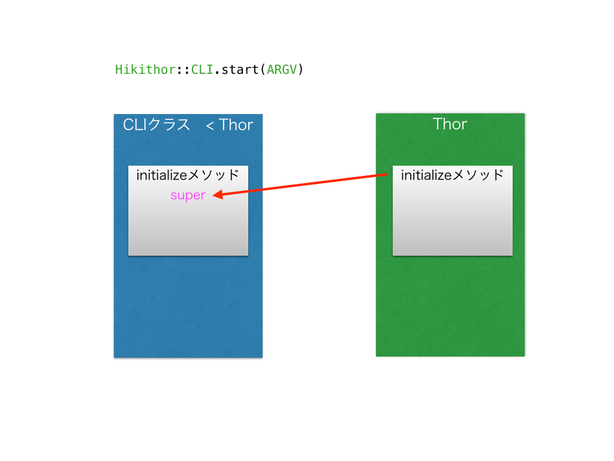
\includegraphics[width=6cm,bb=0 0 442 500]{../figs/./hikiutils_yamane.003.jpg}
\caption{}
\label{default}\end{center}\end{figure}
\begin{enumerate}
\item Hikithor::CLI.start(ARGV)が呼ばれる
\item initializeメソッドが呼ばれる
\item これではThorのinitializeメソッドが呼ばれない
\item superを書くことでThorのinitializeメソッドが呼ばれる
\end{enumerate}
\begin{itemize}
\item optparseの実行コード
\end{itemize}\begin{lstlisting}[style=customRuby]
# -*- coding: utf-8 -*-                                                         
require 'kconv'
require 'hikidoc'
require 'erb'
require "hikiutils/version"
require "hikiutils/tmarshal"
require "hikiutils/infodb"
require 'systemu'
require 'optparse'
require 'fileutils'
require 'yaml'
require 'pp'

module HikiUtils
  DATA_FILE=File.join(ENV['HOME'],'.hikirc')
  attr_accessor :src, :target, :editor_command, :browser, :data_name, :l_dir

  class Command


HTML_TEMPLATE = <<EOS
<!DOCTYPE html                                                                  
    PUBLIC "-//W3C//DTD HTML 4.01 Transitional//EN"                         
    "http://www.w3.org/TR/html4/loose.dtd">                                 
<html lang="ja">                                                            
<html>                                                                      
<head>                                                                      
  <meta http-equiv="Content-Language" content="ja">                         
  <meta http-equiv="Content-Type" content="text/html; charset=UTF-8">       
  <title><%= title %></title>                                               
</head>                                                                     
<body>                                                                      
  <%= body %>                                                               
</body>                                                                     
</html>                                                                     
EOS

    def self.run(argv=[])
      print "hikiutils: provide utilities for helping hiki editing.\n"
      new(argv).execute
    end

    def initialize(argv=[])
      @argv = argv
      @data_name=['nick_name','local_dir','local_uri','global_dir','global_uri']
      data_path = File.join(ENV['HOME'], '.hikirc')
      DataFiles.prepare(data_path)
      read_sources
    end

\end{lstlisting}
\begin{figure}[htbp]\begin{center}
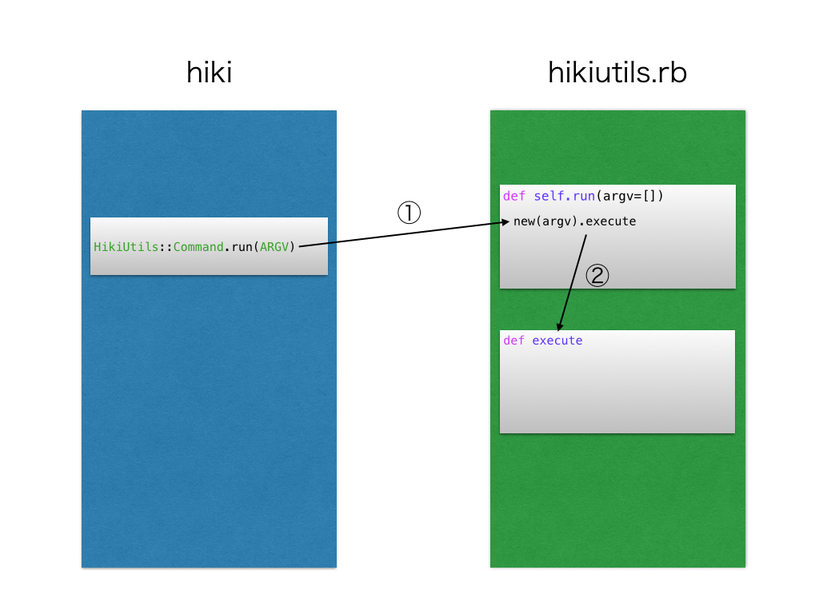
\includegraphics[width=6cm,bb=0 0 442 500]{../figs/./hikiutils_yamane.001.jpg}
\caption{}
\label{default}\end{center}\end{figure}
\begin{enumerate}
\item HikiのHikiUtils::Command.run(ARGV)でhikiutils.rbのrunメソッドを呼ぶ
\item new(argv).executeでexecuteメソッドが実行される
\end{enumerate}
\paragraph{コマンドの表示と実行}
\begin{itemize}
\item Thorのコード
\end{itemize}\begin{lstlisting}[style=customRuby]
    desc 'show,--show', 'show sources'
    map "--show" => "show"
    def show
      printf("target_no:%i\n",@src[:target])
      printf("editor_command:%s\n",@src[:editor_command])
      @i_size,@n_size,@l_size,@g_size=3,5,30,15 #i,g_size are fixed             
      n_l,l_l=0,0
      @src[:srcs].each_with_index{|src,i|
        n_l =(n_l= src[:nick_name].length)>@n_size? n_l:@n_size
        l_l =(l_l= src[:local_dir].length)>@l_size? l_l:@l_size
      }
      @n_size,@l_size=n_l,l_l
      command = Command.new
      header = command.display_format('id','name','local directory','global uri\
',@i_size,@n_size,@l_size,@g_size)

      puts header
      puts '-' * header.size

      @src[:srcs].each_with_index{|src,i|
        target = i==@src[:target] ? '*':' '
        id = target+i.to_s
        name=src[:nick_name]
        local=src[:local_dir]
        global=src[:global_uri]
        puts command.display_format(id,name,local,global,@i_size,@n_size,@l_siz\
e,@g_size)
      }
    end

    desc 'version,--version,-v', 'show program version'
    map "--version" => "version"
    map "-v" => "version"
    def version
      puts HikiUtils::VERSION
    end

    desc 'add,--add', 'add sources info'
    map "--add" => "add"
    option :add
    def add
      cont = {}
      @data_name.each{|name|
        printf("%s ? ", name)
        tmp = STDIN.gets.chomp
        cont[name.to_sym] = tmp
      }
      @src[:srcs] << cont
      show
    end

    desc 'target VAL,--target VAL', 'set target id'
    map "--target" => "target"
    def target(val)
      @src[:target] = val.to_i
      show
    end

    desc 'edit FILE,--edit FILE', 'open file'
    map "--edit" => "edit"
    def edit(file)
      t_file=File.join(@l_dir,'text',file)
      if !File.exist?(t_file) then
        file=File.open(t_file,'w')
        file.close
        File.chmod(0777,t_file)
      end
      p command="#{@editor_command} #{t_file}"
      system command
    end

    desc 'list [FILE],--list [FILE]', 'list files'
    map "--list" => "list"
    def list(file)
      file ='' if file==nil
      t_file=File.join(@l_dir,'text')
      print "target_dir : "+t_file+"\n"
      print `cd #{t_file} ; ls -lt #{file}*`
    end

    desc 'update FILE,--update FILE', 'update file'
    map "--update" => "update"
    def update(file0)
      file = (file0==nil) ? 'FrontPage' : file0
      t_file=File.join(@l_dir,'cache/parser',file)
      FileUtils.rm(t_file,:verbose=>true)
      info=InfoDB.new(@l_dir)
      info.update(file0)
      l_path = @src[:srcs][@target][:local_uri]
      p command="open -a #{@browser} \'#{l_path}/?#{file}\'"
      system command
      p "If you get open error, try rackup from the src_dir."
      p "If you get 整形式になっていません, try login as a valid user."
    end

    desc 'rsync,--rsync', 'rsync files'
    map "--rsync" => "rsync"
    option :rsync
    def rsync
      p local = @l_dir
      p global = @src[:srcs][@target][:global_dir]
      p command="rsync -auvz -e ssh #{local}/ #{global}"
      system command
    end

    desc 'datebase FILE,--database FILE', 'read datebase file'
    map "--database" => "database"
    def database(file_name)
      info=InfoDB.new(@l_dir)
      p info.show(file_name)
    end

    desc 'display FILE,--display FILE', 'display converted hikifile'
    map "--display" => "display"
    def display(file)
      body = HikiDoc.to_html(File.read(file))
      source = HTML_TEMPLATE
      title = File.basename(file)
      erb = ERB.new(source)
      t = File.open(file+".html",'w')
      t.puts(erb.result(binding))
      t.close
      system "open #{t.path}"
    end

    desc 'checkdb,--checkdb', 'check database file'
    map "--checkdb" => "checkdb"
    def checkdb
      result= InfoDB.new(@l_dir).show_inconsist
      print (result=='') ? "db agrees with text dir.\n" : result
    end

    desc 'remove [FILE],--remove [FILE]', 'remove files'
    map "--remove" => "remove"
    def remove(file_name)
      p text_path = File.join(@l_dir,'text',file_name)
      p attach_path = File.join(@l_dir,'cache/attach',file_name)
      begin
        File.delete(text_path)
      rescue => evar
        puts evar.to_s
      end
      begin
        Dir.rmdir(attach_path)
      rescue => evar
        puts evar.to_s
      end

      info=InfoDB.new(@l_dir)
      p "delete "
      del_file=info.delete(file_name)
      info.show_link(file_name)
      info.dump
    end

    desc 'move [FILE],--move [FILE]', 'move file'
    map "--move" => "move"
    def move(files)
      begin
        p file1_path = File.join(@l_dir,'text',files[0])
        p file2_path = File.join(@l_dir,'text',files[1])
      rescue => evar
        puts evar.to_s
        puts "error on move_files, check the input format, especially comma sep\
aration."
        exit
      end
      return if file1_path==file2_path
      if File.exist?(file2_path) then
        print ("moving target #{files[1]} exists.\n")
        print ("first remove#{files[1]}.\n")
        return
      else
        File.rename(file1_path,file2_path)
      end

      info=InfoDB.new(@l_dir)

      db = info.db

      pp file0=db[files[0]]
      db.delete(files[0])
      db[files[1]]=file0
      db[files[1]][:title]=files[1] if db[files[1]][:title]==files[0]
      pp db[files[1]]

      db.each{|ele|
        ref = ele[1][:references]
        if ref.include?(files[0]) then
          p link_file=ele[0]
          link_path = File.join(@l_dir,'text',link_file)

          cont = File.read(link_path)
          if Kconv.iseuc(cont) then
            print "euc\n"
            utf8_cont=cont.toutf8
            utf8_cont.gsub!(/#{files[0]}/,"#{files[1]}")
            cont = utf8_cont.toeuc
          else
            cont.gsub!(/#{files[0]}/,"#{files[1]}")
          end

          File.write(link_path,cont)

          ref.delete(files[0])
          ref << files[1]

          p cache_path = File.join(@l_dir,'cache/parser',link_file)
          begin
            File.delete(cache_path)
          rescue => evar
            puts evar.to_s
          end
        end
      }

      info.dump
    end

    desc 'euc FILE,--euc FILE', 'translate file to euc'
    map "--euc" => "euc"
    def euc(file)
      p file_path = File.join(@l_dir,'text',file)
      cont = File.readlines(file_path)
      cont.each{|line| puts line.toeuc }
    end
  end
\end{lstlisting}
showメソッドからeucメソッドまではコマンドの表示と実行を行う.

\begin{figure}[htbp]\begin{center}
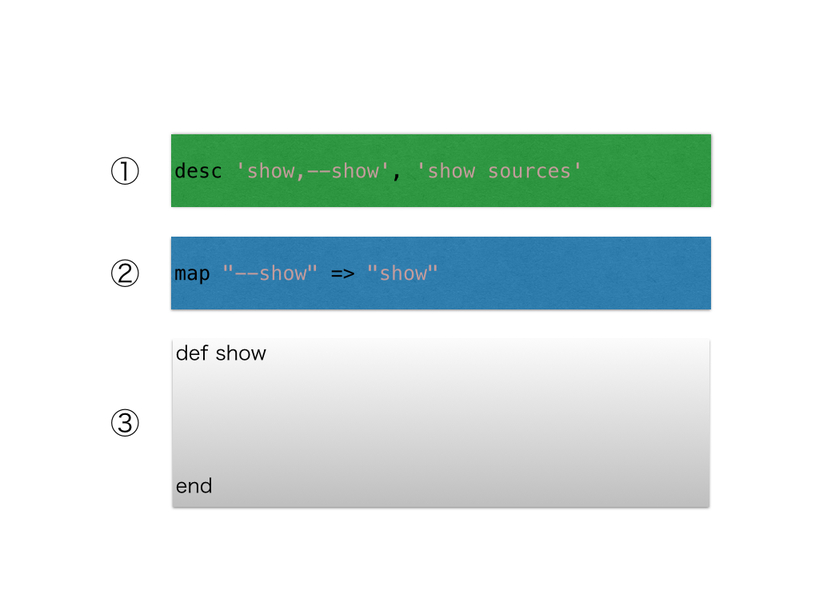
\includegraphics[width=6cm,bb=0 0 442 500]{../figs/./hikiutils_yamane.002.jpg}
\caption{}
\label{default}\end{center}\end{figure}
\begin{enumerate}
\item コマンド名,コマンドの説明を一覧に表示させる
\item パブリックメソッドのコマンドを別のコマンド名でも実行できるようにする
\item コマンドの命令の実行コード
\end{enumerate}
\begin{itemize}
\item optparseのコード
\end{itemize}\begin{lstlisting}[style=customRuby]
    def execute
      @argv << '--help' if @argv.size==0
      command_parser = OptionParser.new do |opt|
        opt.on('-v', '--version','show program Version.') { |v|
          opt.version = HikiUtils::VERSION
          puts opt.ver
        }
        opt.on('-s', '--show','show sources') {show_sources}
        opt.on('-a', '--add','add sources info') {add_sources }
        opt.on('-t', '--target VAL','set target id') {|val| set_target(val)}
        opt.on('-e', '--edit FILE','open file') {|file| edit_file(file) }
        opt.on('-l', '--list [FILE]','list files') {|file| list_files(file)}
        opt.on('-u', '--update FILE','update file') {|file| update_file(file) }
        opt.on('-r', '--rsync','rsync files') {rsync_files}
        opt.on('--database FILE','read database file') {|file| db_file(file)}
        opt.on('--display FILE','display converted hikifile') {|file| display(file)}
        opt.on('-c', '--checkdb','check database file') {check_db}
        opt.on('--remove FILE','remove file') {|file| remove_file(file)}
        opt.on('--move FILES','move file1,file2',Array) {|files| move_file(files)}
        opt.on('--euc FILE','translate file to euc') {|file| euc_file(file)}
        opt.on('--initialize','initialize source directory') {dir_init() }
      end
      begin
        command_parser.parse!(@argv)
      rescue=> eval
        p eval
      end
      dump_sources
      exit
    end    
    
    def dir_init()
      begin
        p target_dir = File.readlines('./.hikirc')[0]
      rescue
        p target_dir=@src[:srcs][@target][:local_dir]
        File.open('./.hikirc','w'){|file| file.print "#{target_dir}\n"}
      end
      cp_files=[['Rakefile_hiki_sync','Rakefile'],
                ['hiki_help.yml','hiki_help.yml']]
      cp_files.each{|files|
        p source = File.join(File.expand_path('..', __FILE__),'templates',files[0])
        p target = File.join(Dir.pwd,files[1])
        FileUtils.cp(source,target,:verbose=>true)
      }
      ['figs','data'].each{|dir|
        begin
          Dir.mkdir(dir)
        rescue => e
          print e
        end
      }
      begin
        p cont=File.read('./.gitignore')
        unless cont.include?('.hikirc')
          File.open('./.gitignore','w'){|file| file.print(".hikirc\n")}
        end
      rescue
        File.open('./.gitignore','w'){|file| file.print(".hikirc\n")}
      end
    end

    def display(file)
      body = HikiDoc.to_html(File.read(file))
      source = HTML_TEMPLATE
      title = File.basename(file)
      erb = ERB.new(source)
      t = File.open(file+".html",'w')
      t.puts(erb.result(binding))
      t.close
      system "open #{t.path}"
    end

    def euc_file(file)
      p file_path = File.join(@l_dir,'text',file)
      cont = File.readlines(file_path)
      cont.each{|line| puts line.toeuc }
    end

    def move_file(files)
      begin
        p file1_path = File.join(@l_dir,'text',files[0])
        p file2_path = File.join(@l_dir,'text',files[1])
      rescue => evar
        puts evar.to_s
        puts "error on move_files, check the input format, especially comma separation."
        exit
      end
      return if file1_path==file2_path
      if File.exist?(file2_path) then
        print ("moving target #{files[1]} exists.\n")
        print ("first remove#{files[1]}.\n")
        return
      else
        File.rename(file1_path,file2_path)
      end

      info=InfoDB.new(@l_dir)

      db = info.db

      pp file0=db[files[0]]
      db.delete(files[0])
      db[files[1]]=file0
      db[files[1]][:title]=files[1] if db[files[1]][:title]==files[0]
      pp db[files[1]]

      db.each{|ele|
        ref = ele[1][:references]
        if ref.include?(files[0]) then
          p link_file=ele[0]
          link_path = File.join(@l_dir,'text',link_file)

          cont = File.read(link_path)
          if Kconv.iseuc(cont) then
            print "euc\n"
            utf8_cont=cont.toutf8
            utf8_cont.gsub!(/#{files[0]}/,"#{files[1]}")
            cont = utf8_cont.toeuc
          else
            cont.gsub!(/#{files[0]}/,"#{files[1]}")
          end

          File.write(link_path,cont)

          ref.delete(files[0])
          ref << files[1]

          p cache_path = File.join(@l_dir,'cache/parser',link_file)
          begin
            File.delete(cache_path)
          rescue => evar
            puts evar.to_s
          end
        end
      }

      info.dump
    end

    def remove_file(file_name)
      p text_path = File.join(@l_dir,'text',file_name)
      p attach_path = File.join(@l_dir,'cache/attach',file_name)
      begin
        File.delete(text_path)
      rescue => evar
        puts evar.to_s
      end
      begin
        Dir.rmdir(attach_path)
      rescue => evar
        puts evar.to_s
      end

      info=InfoDB.new(@l_dir)
      p "delete "
      del_file=info.delete(file_name)
      info.show_link(file_name)
      info.dump
    end

    def check_db
      result= InfoDB.new(@l_dir).show_inconsist
      print (result=='') ? "db agrees with text dir.\n" : result
    end

    def db_file(file_name)
      info=InfoDB.new(@l_dir)
      p info.show(file_name)
    end

    def rsync_files
      p local = @l_dir
      p global = @src[:srcs][@target][:global_dir]
#"/Users/bob/Sites/nishitani0/Internal/data"                                 
#"bob@dmz0:/Users/bob/nishitani0/Internal/data"                              
#      p command="rsync -auvz -e ssh #{local}/ #{global}"                    
      p command="rsync -auvz -e ssh #{local}/ #{global}"
#  system 'rsync -auvz -e ssh ~/Sites/nishitani0 bob@nishitani0.kwansei.ac.jp:Sites/'                                                                    
      system command
    end

    def update_file(file0)
      file = (file0==nil) ? 'FrontPage' : file0
      #rm cache file                                                         
      t_file=File.join(@l_dir,'cache/parser',file)
      begin
        FileUtils.rm(t_file,:verbose=>true)
      #update info file                                                      
      info=InfoDB.new(@l_dir)
      info.update(file0)

      rescue
        print "some errors on touch, but dont mind...\n"
      end

      #open file on browser                                                  
      l_path = @src[:srcs][@target][:local_uri]
#      p command="open -a #{@browser} \'#{l_path}/?c=edit;p=#{file}\'"       
      p command="open -a #{@browser} \'#{l_path}/?#{file}\'"
      system command
      p "If you get open error, try rackup from the src_dir."
      p "If you get 整形式になっていません, try login as a valid user."
    end

    def list_files(file)
      file ='' if file==nil
      t_file=File.join(@l_dir,'text')
      print "target_dir : "+t_file+"\n"
      print `cd #{t_file} ; ls -lt #{file}*`
    end

    def edit_file(file)
      t_file=File.join(@l_dir,'text',file)
      if !File.exist?(t_file) then
        file=File.open(t_file,'w')
        file.close
        File.chmod(0777,t_file)
      end
      p command="#{@editor_command} #{t_file}"
      system command
    end

    def dump_sources
      file = File.open(DATA_FILE,'w')
      YAML.dump(@src, file)
      file.close
    end

    def set_target(val)
      @src[:target] = val.to_i
      show_sources
    end

    def show_sources()
      printf("target_no:%i\n",@src[:target])
      printf("editor_command:%s\n",@src[:editor_command])
      check_display_size()
      header = display_format('id','name','local directory','global uri')

      puts header
      puts '-' * header.size

      @src[:srcs].each_with_index{|src,i|
        target = i==@src[:target] ? '*':' '
        id = target+i.to_s
        name=src[:nick_name]
        local=src[:local_dir]
        global=src[:global_uri]
        puts display_format(id,name,local,global)
      }

    end

    def check_display_size
      @i_size,@n_size,@l_size,@g_size=3,5,30,15 #i,g_size are fixed          
      n_l,l_l=0,0
      @src[:srcs].each_with_index{|src,i|
        n_l =(n_l= src[:nick_name].length)>@n_size? n_l:@n_size
        l_l =(l_l= src[:local_dir].length)>@l_size? l_l:@l_size
      }
      @n_size,@l_size=n_l,l_l
    end

    def display_format(id, name, local, global)
      name_length  = @n_size-full_width_count(name)
      local_length = @l_size-full_width_count(local)
      global_string= global.size < @g_size ? global : global[0..@g_size]
      [id.to_s.rjust(@i_size), name.ljust(name_length),
               local.ljust(local_length),
                          global_string.ljust(@g_size)].join(' | ')
    end

    def full_width_count(string)
      string.each_char.select{|char| !(/[ -~。-゚]/.match(char))}.count
    end

    def add_sources
      cont = {}
      @data_name.each{|name|
        printf("%s ? ", name)
        tmp = gets.chomp
        cont[name.to_sym] = tmp
      }
      @src[:srcs] << cont
      show_sources
    end

    def read_sources
      file = File.open(DATA_FILE,'r')
      @src = YAML.load(file.read)
      file.close
      @target = @src[:target]
      @l_dir=@src[:srcs][@target][:local_dir]
      browser = @src[:browser]
      @browser = (browser==nil) ? 'firefox' : browser
      p editor_command = @src[:editor_command]
      @editor_command = (editor_command==nil) ? 'open -a mi' : editor_command
    end
  end
end
\end{lstlisting}
displayメソッドからadd\_sourcesメソッドまではoptで登録されたコマンドの実行コードが書かれている.

